%%===========================================================%%
%%                                                           %%
%%                        CORRECTIONS                        %%
%%                                                           %%
%%===========================================================%%


\chapter{Corrections}\label{chap:corrections}

\section{Method of corrections application}\label{sec:correctionProcedure}
\begin{equation}
  \frac{d\sigma}{dq} = \frac{1}{\Delta q} \times \frac{1}{\varepsilon} \times \frac{N^{\mathit{w}}-N^{\mathit{w}}_\textrm{bkgd}}{\mathit{L}_{\textrm{int}}^{\textrm{eff}}}
\end{equation}

%remembed about accounting for RP trigger eff!!!
\begin{equation}\label{eq:effectiveLumi}
	\mathit{L}_{\textrm{int}}^{\textrm{eff}} = \sum\limits_{\textrm{run}}\mathit{L}_{\textrm{int}}^{\textrm{run}} \times \epsilon_{\textrm{veto}}(L^{\textrm{run}})
\end{equation}
% \left(\epsilon_{\textrm{veto}}^{\textrm{online}} \oplus \epsilon_{\textrm{veto}}^{\textrm{offline}}(L_{\textrm{run}}) \right)

\begin{equation}
	\varepsilon = \epsilon_{\textrm{\tiny ET/IT}} \times \epsilon_{\textrm{vrtx}}(q) \times \epsilon_{\ref{enum:CutZVx}} \times \epsilon_{\ref{enum:CutDeltaZVx}} \times \epsilon_{\ref{enum:CutMissingPt}} \times \epsilon_{\textrm{\tiny PID}}(q)
\end{equation}

\begin{equation}
	N^{\mathit{w}} = \sum\limits_{\textrm{event}}\mathit{w}_{\textrm{event}}
\end{equation}



\begin{equation}
	\mathit{w} = \left[\prod\limits_{\textrm{sign}} \epsilon_{\textrm{\tiny TOF}}(\textrm{sign}, \textrm{PID}, p_{T},z_{vx},\eta)  \times \prod\limits_{\textrm{sign}} \epsilon_{\textrm{\tiny TPC}}(\textrm{sign}, \textrm{PID}, p_{T},z_{vx},\eta) \times \prod\limits_{\textrm{side}}\epsilon_{\textrm{\tiny RP}}^{\textrm{side}}(p_{x},p_{y}) \right]^{-1},
\end{equation}
\[\textrm{sign}\in\{+,-\},~~\textrm{side}\in\{E,W\}\]
% ()




\section{Acceptances and efficiencies}

In this section we present calculation of all efficiencies except TPC track reconstruction and TOF hit reconstruction and matching efficiency, which were discussed and presented in Ref.~\cite{supplementaryNote}.

\subsection{Trigger efficiency}\label{sec:triggerEff}
\subsubsection{Online veto (BBC-small and ZDC veto)}\label{sec:onlineVetoEff}

Vetoeing signal in BBC-small and ZDC detectors on both sides of STAR was implemented in the logic of RP\_CPT2 trigger. Common correction of the online and offline vetoes which is used in the correction procedure explained in Sec.~\ref{sec:correctionProcedure} is presented in. Sec.~\ref{sec:offlineVetoEff}. However, to help quantifiy effect of just the online vetoes in BBC-small and ZDCs we show the Fig.~\ref{fig:onlineVetoEff} with the efficiency of the joint BBC-small and ZDC veto as a function of the instantaneous luminosity calculated from the zero-bias data. Details of the way the efficiency was calculated as well as description of the data in the Figure is the same as explained in Sec.~\ref{sec:onlineAndOfflineVetoEff}.
%---------------------------
\begin{figure}[ht!]
\centering%
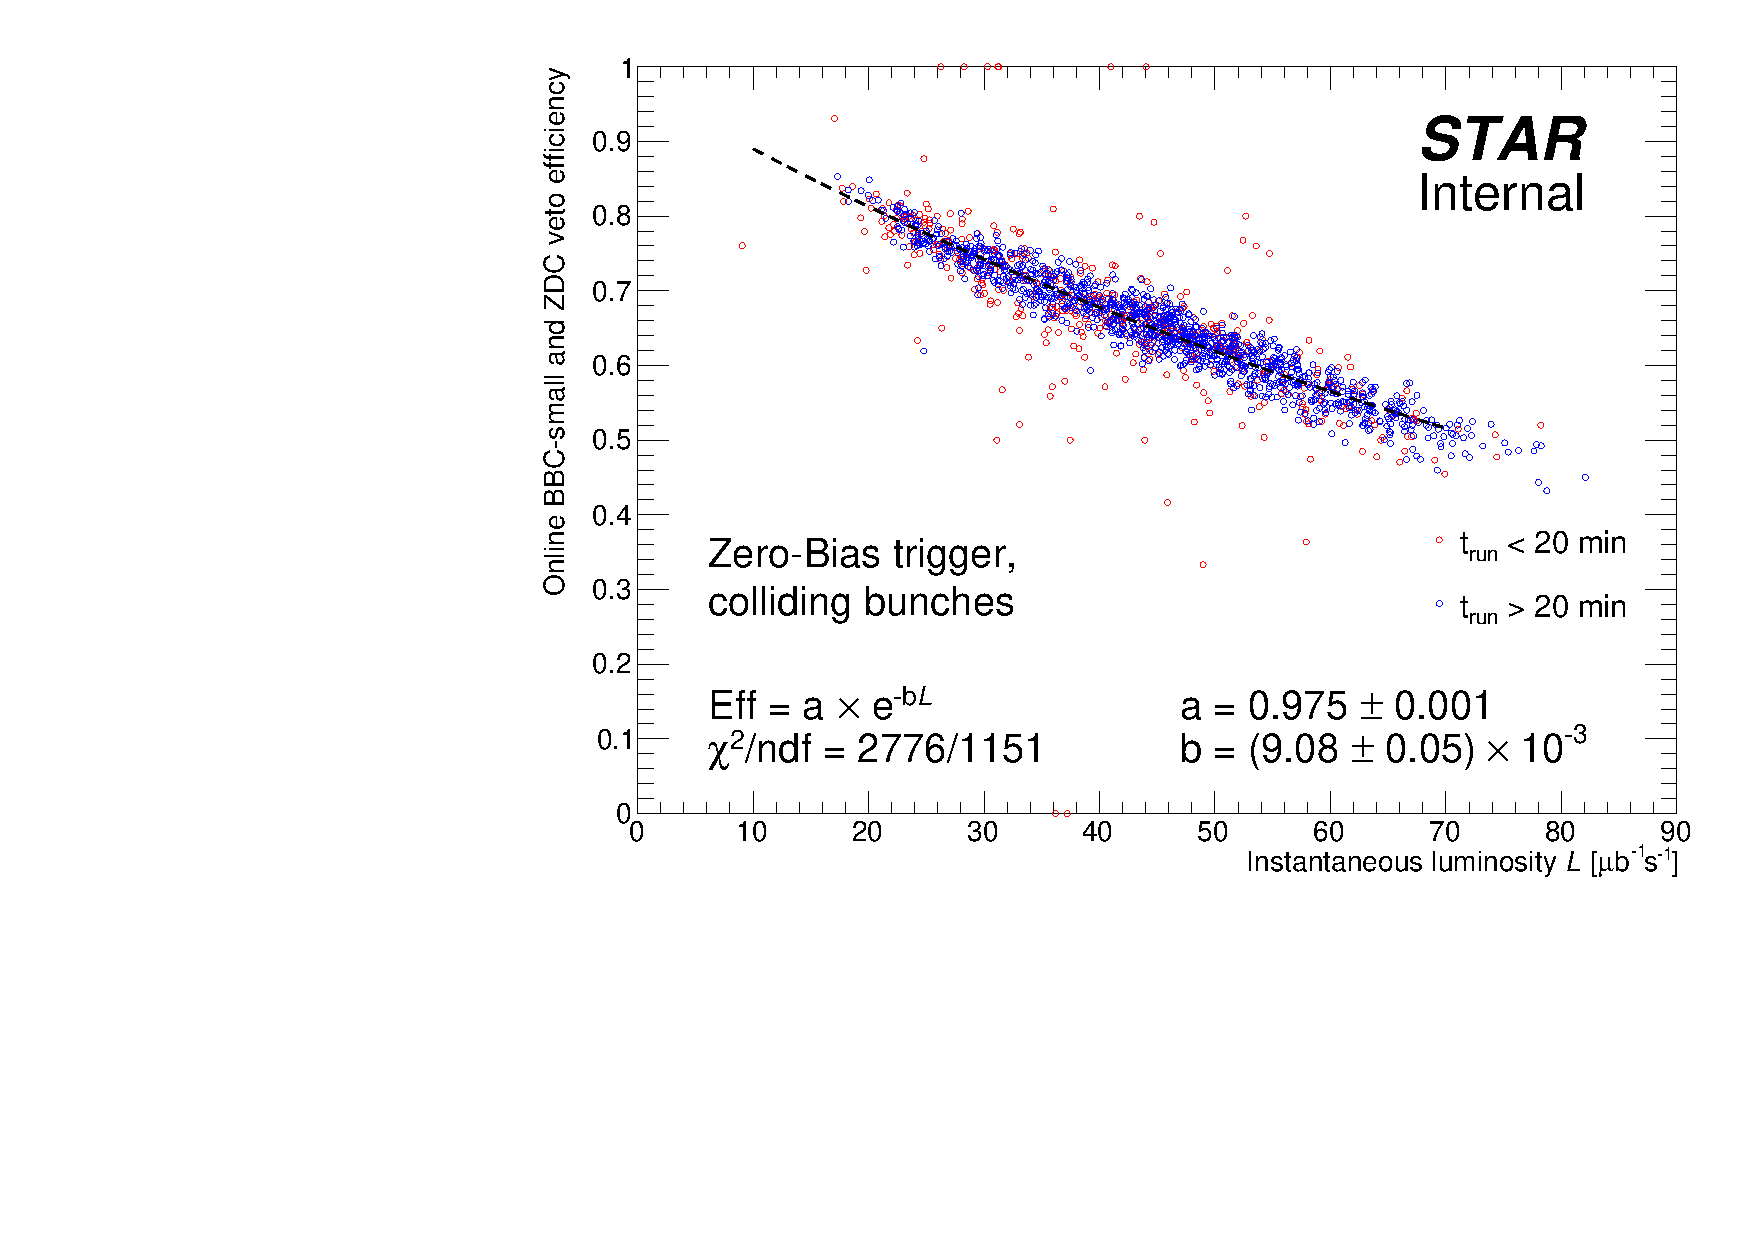
\includegraphics[width=0.65\linewidth,page=1]{graphics/corrections/OnlineVetoEffVsInstLumi_graph.pdf}%
\caption{Overall efficiency of the online BBC-small and ZDC veto as a function of instantaneous luminosity.}\label{fig:onlineVetoEff}%
\end{figure}
%---------------------------

\subsubsection{RP triggering efficiency}\label{sec:rpTrigEff}

Based on preliminary studies preformed during data taking using fast offline data (MuDst) we concluded that the RP triggering efficiency is very close to 100~\% and eventual correction (which is going to be evaluated) is much smaller than overall systematic uncertainty. For the time being we assume that
\begin{equation}
\mbox{\LARGE$\varepsilon$}\left(\TRE\land\TRW\right) =  \mbox{\LARGE$\varepsilon$}\left(\TRW\right) \times \mbox{\LARGE$\varepsilon$}\left(\TRE\right) = 1.
\end{equation}


% Wydajnosc samego trygerowania
% \begin{equation}
% \mbox{\LARGE$\varepsilon$}\left(\TRE\land\TRW\right) = \mbox{\LARGE$\varepsilon$}\left(\TRE\right) \times \mbox{\LARGE$\varepsilon$}\left(\TRW\right),
% \end{equation}
% \begin{equation}
% \mbox{\LARGE$\varepsilon$}\left(\TRE\right) = \mbox{\LARGE$\varepsilon$}\left(\TRE_{1}\vee\TRE_{2}\right),~~~~\mbox{\LARGE$\varepsilon$}\left(\TRW\right) = \mbox{\LARGE$\varepsilon$}\left(\TRW_{1}\vee\TRW_{2}\right),
% \end{equation}
% dobrze bedzie policzyc już z danych, najlepiej elastycznych (ale można też z CD) patrzac jak czesto stacje z dobrymi sladami maja sygnal trygerowy.
% 
% \begin{equation}\begin{split}
% \mbox{\LARGE$\varepsilon$}\left(\TRW\right) = \mbox{\LARGE$\varepsilon$}\left(\TRW\left|\RPE\&\RPW\&~!\TRNE\&~!\TRNW\right.\right) = \mbox{\LARGE$\varepsilon$}\left(\TRW_{1}\vee\TRW_{2}\left|\RPE\&\RPW\&~!\TRNE\&~!\TRNW\right.\right)=\\
% =\mbox{\LARGE$\varepsilon$}\left(\TRW_{1}\left|\RPE\&\RPW\&~!\TRNE\&~!\TRNW\right.\right)+\mbox{\LARGE$\varepsilon$}\left(\TRW_{2}\left|\RPE\&\RPW\&~!\TRNE\&~!\TRNW\right.\right)+\\-\mbox{\LARGE$\varepsilon$}\left(\TRW_{1}\land\TRW_{2}\left|\RPE\&\RPW\&~!\TRNE\&~!\TRNW\right.\right)~~~~~\text{(analogicznie po stronie EAST)}
% \end{split}\end{equation}


\subsubsection{Up and Down RP combination veto (due to dead material)}\label{sec:rpDeadMat}

Probability that secondaries induced by proton with successfully reconstructed and selected RP track generate a trigger signal in the other RP branch on the same side was calculated using the embedded MC (see Sec.~6.3 in Ref.~\cite{supplementaryNote} for details of RP simulation in Geant4). Forward protons from CEP process provided by GenEx~\cite{GenEx} were simultaneously generated from the interaction point spatially distributed the same as in the data. MC samples for all runs with RP\_CPT2 triggers were produced to account for non-constant positions of the RP detectors throughout the run 15. Number of simulated events for each run was proportional to number of RP\_CPT2 triggers in given run. The angular divergence of the beams was also simulated.

The discussed probability, $\mathcal{P}_{\text{DM~veto}}^{\text{side}}$, was calculated as a probability that a MC-trigger signal is present in the branch on given side other than east and west branches where primary forward protons are expected from their initial momenta, under condition that these east and west branches detect a MC-trigger signal and there is no veto due to simultaneous ET\&IT trigger bits in the overlayed data (no pile-up veto). By MC-trigger we understand the trigger signal reconstructed solely from the simulated data (not from the data embedded into).

Technically the $\mathcal{P}_{\text{DM~veto}}^{\text{side}}$ was obtained in the following procedure:
\begin{enumerate}
  \item No simultaneous ET\&IT trigger bits were allowed in the data of an event that simulated signal was embedded into.
	\item It was verified if there are MC-trigger signals in east and west branches that the primary forward protons were expected to reach based on their $p_{y}$ ($p_{y}>0$ - branch UP, $p_{y}<0$ - branch DOWN). These events formed $set~A$.
	\item Events with the MC-trigger signal in RP branch other than the branch with MC-trigger signal expected from proton $p_{y}$ on given side formed $set~B$.
	\item The probability was determined by the ratio of histograms from $set~B$ and $set~A$:
	\begin{equation}\label{eq:rpDeadMatProb}
	\begin{split}
 \mathcal{P}_{\text{DM~veto}}^{\text{side}}(p_{x}, p_{y}, z_{\text{vtx}}) = \mbox{\LARGE$\varepsilon$}^{\text{side}}\left(\Vdm\left|!\Vpu\land\TRE\land\TRW\right.\right) = ~~~~~~~~~~~~~~~~~~~~~~~~~~~~~~~~~~~~~~\\~~~~~~~~~~~~~~~~~~~~~~~~~~~~~~~ =%
 \frac{(p_{x}, p_{y}, z_{\text{vtx}})~\text{histogram for protons from}~set~B}{(p_{x}, p_{y}, z_{\text{vtx}})~\text{histogram for protons from}~set~A}
 \end{split}
  \end{equation}
	
\end{enumerate}

It should be noted that the momentum components $(p_{x}, p_{y})$ were taken from the proton with accounted effect of the beam divergence (after the original initial momentum smearing). Sample probability of a dead-material-induced veto is shown in Fig.~\ref{fig:sampleRpDeadMatVeto}, with all the remaining results contained in Appendix~\ref{appendix:rpEff}.

The efficiency of the discussed veto which is finally used to correct the data is opposite of the veto probability, namely
\begin{equation}
 \mbox{\LARGE$\epsilon$}_{\text{DM~veto}}^{\text{side}} = 1 - \mathcal{P}_{\text{DM~veto}}^{\text{side}}.
\end{equation}


%---------------------------
\begin{figure}[ht!]
\centering%
\parbox{0.4725\textwidth}{%
  \centering%
  \includegraphics[width=\linewidth,page=3]{graphics/corrections/mcDeadMatProbPxPy.pdf}\label{fig:sampleDeadMatVetoProb}
}%
\quad%
\parbox{0.4725\textwidth}{%
    \caption[Sample probability of ET\&IT trigger veto due to forward proton interaction with dead material.]{Sample probability of ET\&IT trigger veto due to forward proton interaction with dead material. Results were obtained from forward proton MC simulation embedded into zero-bias data.}\label{fig:sampleRpDeadMatVeto}%
}
\end{figure}
%---------------------------





\subsection{Selection efficiency}\label{sec:cutsEff}
\subsubsection{TPC \texorpdfstring{$z$}{z}-vertex cut~(\ref{enum:CutZVx})}
\subsubsection{TPC-RP \texorpdfstring{$z$}{z}-vertex matching~(\ref{enum:CutDeltaZVx})}
\subsubsection{Primary vertices limit~(\ref{enum:CutPrimVx}), BBC-large veto~(\ref{enum:CutBbcLarge}), TOF clusters limit~(\ref{enum:CutTofClusters}) and Up and Down RP combination veto (due to pile-up)}\label{sec:onlineAndOfflineVetoEff}

Combined efficiency of the online veto in BBC-small and ZDC (Sec.~\ref{sec:onlineVetoEff}) and offline cuts (vetoes) on extra TPC-TOF vertices, extra TOF clusters, signal in BBC-large and simultaneous signal in Up and Down RPs, was calculated using the zero-bias data. For each run a fraction of events (for colliding bunches) was calculated in which all mentioned cuts would be satisfied in case of the CEP $\pi^{+}\pi^{-}$/$K^{+}K^{-}$/$p\bar{p}$ event (event would not be vetoed). One can tranform this prescription to simple formula below:

\begin{equation}
 \mbox{\LARGE$\epsilon$}^{\text{veto}}_{b_{E}b_{W}}=\dfrac{\splitdfrac{~~~~~\text{\#events in the run without TOF vertices, without signal in BBC-S, BBC-L, ZDC,}}{\text{RP branches other than} ~b_{E},~b_{W},~\text{and with no more than 1 reconstructed TOF cluster}}}{\text{\#events in the run}}
\end{equation}

In Fig.~\ref{fig:onlineAndOfflineVetoEff} this efficiency is presented as a function instantaneous luminosity delivered by the machine, for each combination of east and west RP branches. Result for each combination is nearly identical as the effect of ET\&IT trigger veto in RPs is not dominant, as well as trigger in all branches had similar acceptance. The data points were fitted with the exponential function (of the form containted in the figure) which reflects the fact that this efficiency should behave similar to the probability of lack of any interaction in the bunch crossing given by the Poisson distribution:
\begin{equation}\label{eq:poisson}
 \text{Pois}(0;\mu) = \frac{\mu^{0}}{0!} \times e^{-\mu} = e^{-\mu}.
\end{equation}
Comparison of the $\mu$ in Eq.~\eqref{eq:poisson} with the fit parameters in Fig.~\ref{fig:onlineAndOfflineVetoEff} leads to approximate determination of the average interaction probability per bunch crossing equal $0.2-0.9$. The result of the fit, $ \mbox{\LARGE$\epsilon$}^{\text{veto}}_{b_{E}b_{W}}(\mathcal{L})$, is finally used to correct measured data as described in Sec.~\ref{sec:correctionProcedure}. 

%---------------------------
\begin{figure}[h]
\centering
\parbox{0.4725\textwidth}{
  \centering
  \begin{subfigure}[b]{\linewidth}
                \subcaptionbox{\label{fig:sampleBbcSmallAdcVsTac}}{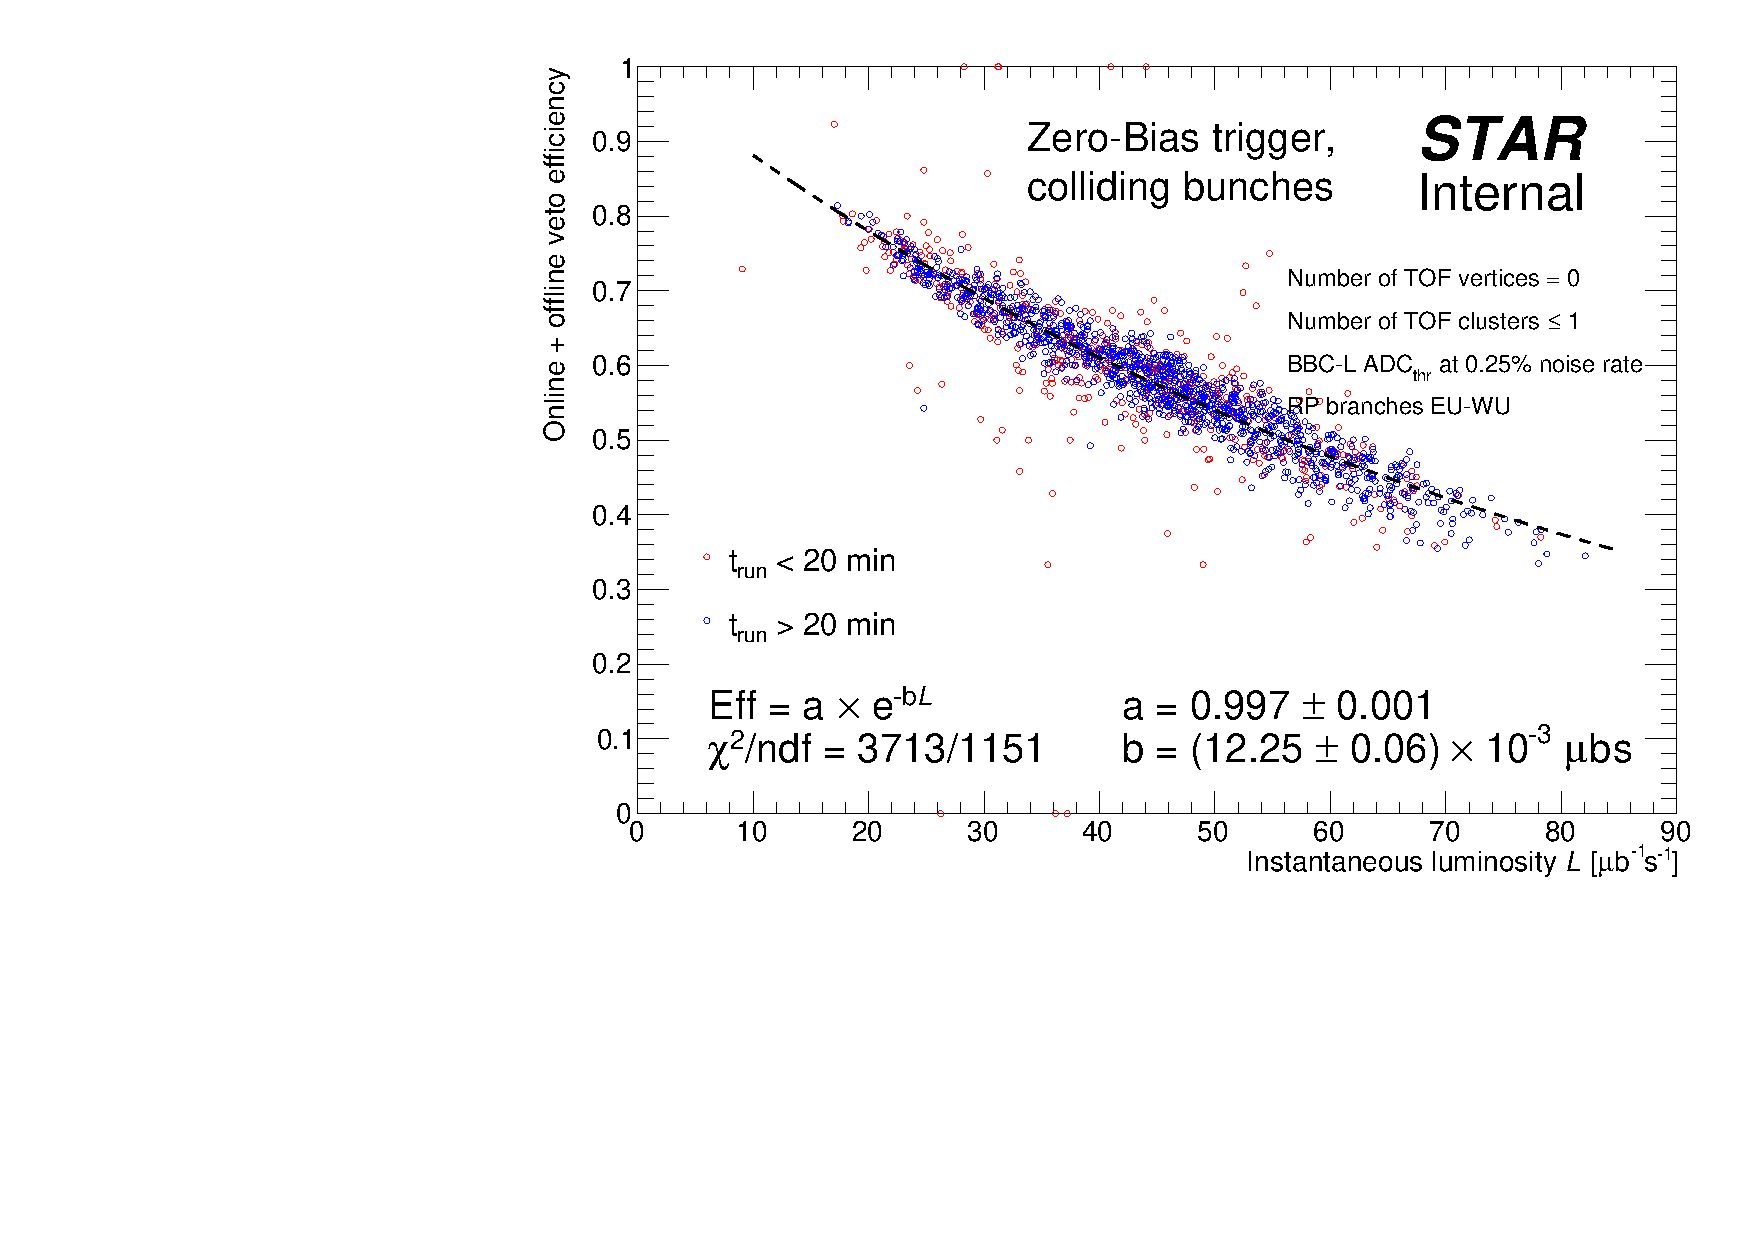
\includegraphics[width=\linewidth,page=1]{graphics/corrections/FullVetoEffVsInstLumi.pdf}}
  \end{subfigure}\\
  \begin{subfigure}[b]{\linewidth}\addtocounter{subfigure}{1}
                \subcaptionbox{\label{fig:sampleBbcSmallAdc}}{\includegraphics[width=\linewidth,page=3]{graphics/corrections/FullVetoEffVsInstLumi.pdf}}
  \end{subfigure}
}%
\quad\quad%
\parbox{0.4725\textwidth}{
  \centering
  \begin{subfigure}[b]{\linewidth}\addtocounter{subfigure}{-2}
                \subcaptionbox{\label{fig:sampleBbcLargeAdcVsTac}}{\includegraphics[width=\linewidth,page=2]{graphics/corrections/FullVetoEffVsInstLumi.pdf}}
  \end{subfigure}\\
  \begin{subfigure}[b]{\linewidth}\addtocounter{subfigure}{1}
                \subcaptionbox{\label{fig:sampleBbcLargeAdc}}{\includegraphics[width=\linewidth,page=4]{graphics/corrections/FullVetoEffVsInstLumi.pdf}}
  \end{subfigure}
}%
\caption[Overall efficiency of online and offlince cuts as a function of instantaneous luminosity.]{Overall efficiency of the online BBC-small, ZDC and ET\&IT trigger veto, primary vertices limit~(\ref{enum:CutPrimVx}), BBC-large veto~(\ref{enum:CutBbcLarge}) and TOF clusters limit~(\ref{enum:CutTofClusters}) as a function of instantaneous luminosity for all possible combinations of east and west RP branches. Red and blue points represent runs lasting for less and more than 20 minutes, respectively. Black dotted lines reprent fits of exponential functions to blue points.}\label{fig:onlineAndOfflineVetoEff}%
\end{figure}
%---------------------------



\subsubsection{Missing \texorpdfstring{$p_{T}$}{pT} cut~(\ref{enum:CutMissingPt})}
\subsubsection{Particle identification~(\ref{enum:CutPid})}


%---------------------------
\begin{figure}[ht!]
\centering
\parbox{0.315\textwidth}{
  \centering
  \begin{subfigure}[b]{\linewidth}{
                \subcaptionbox{\label{fig:sqMassTof_DataVsMC_pion}}{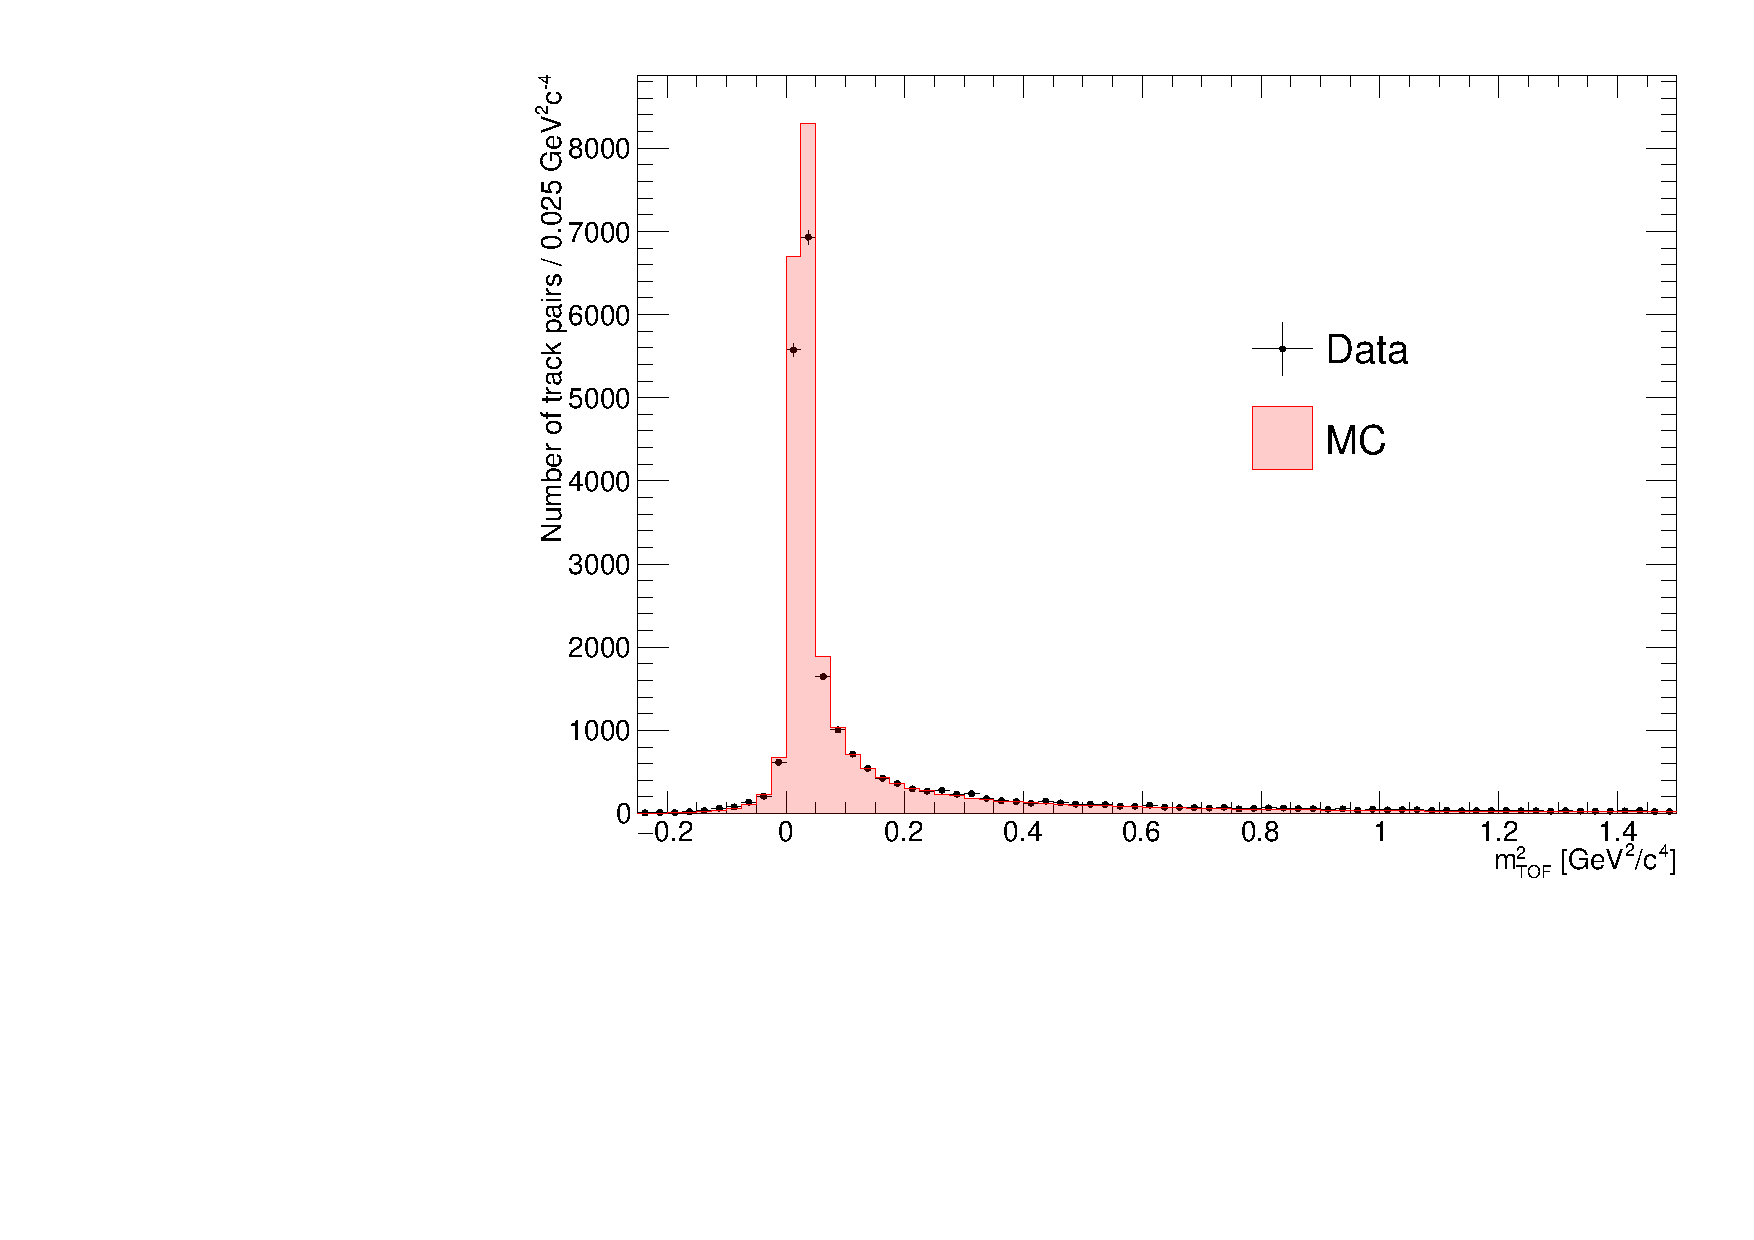
\includegraphics[width=\linewidth,page=1]{graphics/corrections/sqMassTof_DataVsMC.pdf}}}
  \end{subfigure}
}
\quad
\parbox{0.315\textwidth}{
  \centering
  \begin{subfigure}[b]{\linewidth}{
                \subcaptionbox{\label{fig:sqMassTof_DataVsMC_kaon}}{\includegraphics[width=\linewidth,page=2]{graphics/corrections/sqMassTof_DataVsMC.pdf}}}
  \end{subfigure}
}
\quad
\parbox{0.315\textwidth}{
  \centering
  \begin{subfigure}[b]{\linewidth}{
                \subcaptionbox{\label{fig:sqMassTof_DataVsMC_proton}}{\includegraphics[width=\linewidth,page=3]{graphics/corrections/sqMassTof_DataVsMC.pdf}}}
  \end{subfigure}
}%
\caption{Comparison of $m^{2}$ from TOF between data and MC for exclusive $\pi^{+}\pi^{-}$, $K^{+}K^{-}$ and $p\bar{p}$.}
\end{figure}
%---------------------------









\subsection{RP track acceptance and reconstruction efficiency}\label{sec:rpAccAndEff}

To calculate RP acceptance and track reconstruction efficiency the embedded MC technique was used. The same sample was used as that described in Sec.~\ref{sec:rpDeadMat}, used for calculation of the dead-material related trigger veto.

The joint RP acceptance and track reconstruction efficiency for a given STAR side, $\epsilon_{\text{RP}}^{\text{side}}$, was calculated as a probability that a single good quality RP track (satisfying cuts~\ref{enum:RpQualityCuts}-\ref{enum:RpLocalAngles}) matched with true-level primary forward proton is reconstructed on given side in the branch expected based on sign of $p_{y}$ of the proton, under condition that there is a trigger signal in that branch and there is no trigger signal in the other branch on the same side.

Technically the $\epsilon_{\text{RP}}^{\text{side}}$ was obtained in the following procedure:
\begin{enumerate}
	\item It was verified if there is a trigger signal in the branch that the primary forward proton is expected to reach based on its $p_{y}$ ($p_{y}>0$ - branch UP, $p_{y}<0$ - branch DOWN). Additionally required lack of trigger signal in the other branch on the same side. These events formed $set~A$.
	\item The nominal RP track selection algorithm was used to find a single good quality track (cuts~\ref{enum:RpQualityCuts}-\ref{enum:RpLocalAngles}) on given side. If exactly one such track was found, it was additionally checked if it is matched with true-level primary proton. These events formed $set~B$.
	\item The efficiency was determined by the ratio of histograms from $set~B$ and $set~A$:
	\begin{equation}\label{eq:rpEffDef}
 \epsilon_{\text{RP}}^{\text{side}}(p_{x}, p_{y}, z_{\text{vtx}}) = \mbox{\LARGE$\varepsilon$}\left(\RPSIDE\left|\TRSIDE\land~!\TRNSIDE\right.\right) = %
 \frac{(p_{x}, p_{y}, z_{\text{vtx}})~\text{histogram for protons from}~set~B}{(p_{x}, p_{y}, z_{\text{vtx}})~\text{histogram for protons from}~set~A}
  \end{equation}
	
\end{enumerate}

It should be noted that the momentum components $(p_{x}, p_{y})$ were taken from the proton with accounted effect of the beam divergence (after the original initial momentum smearing).

%---------------------------
\begin{figure}[ht!]%
\centering%
\begin{minipage}{.4725\textwidth}%
  \centering%
  \includegraphics[width=\linewidth,page=10]{graphics/corrections/mcFullEffPxPy.pdf}%
  \caption[Sample RP track reconstruction efficiency in a single $z$-vertex bin.]{Sample RP track reconstruction efficiency in a single $z$-vertex bin on the east STAR side. The efficiency was calculated using forward proton MC simulation embedded into zero-bias data. Green envelopes mark the fiducial region of the measurement, while dashed yellow lines mark the part of the fiducial region with a data-driven efficiency correction needed, as explained in Sec.~10.3.1 of Ref.~\cite{supplementaryNote}.}\label{fig:rpEffSample}
\end{minipage}%
\quad\quad%
\begin{minipage}{.4725\textwidth}%
  \centering
  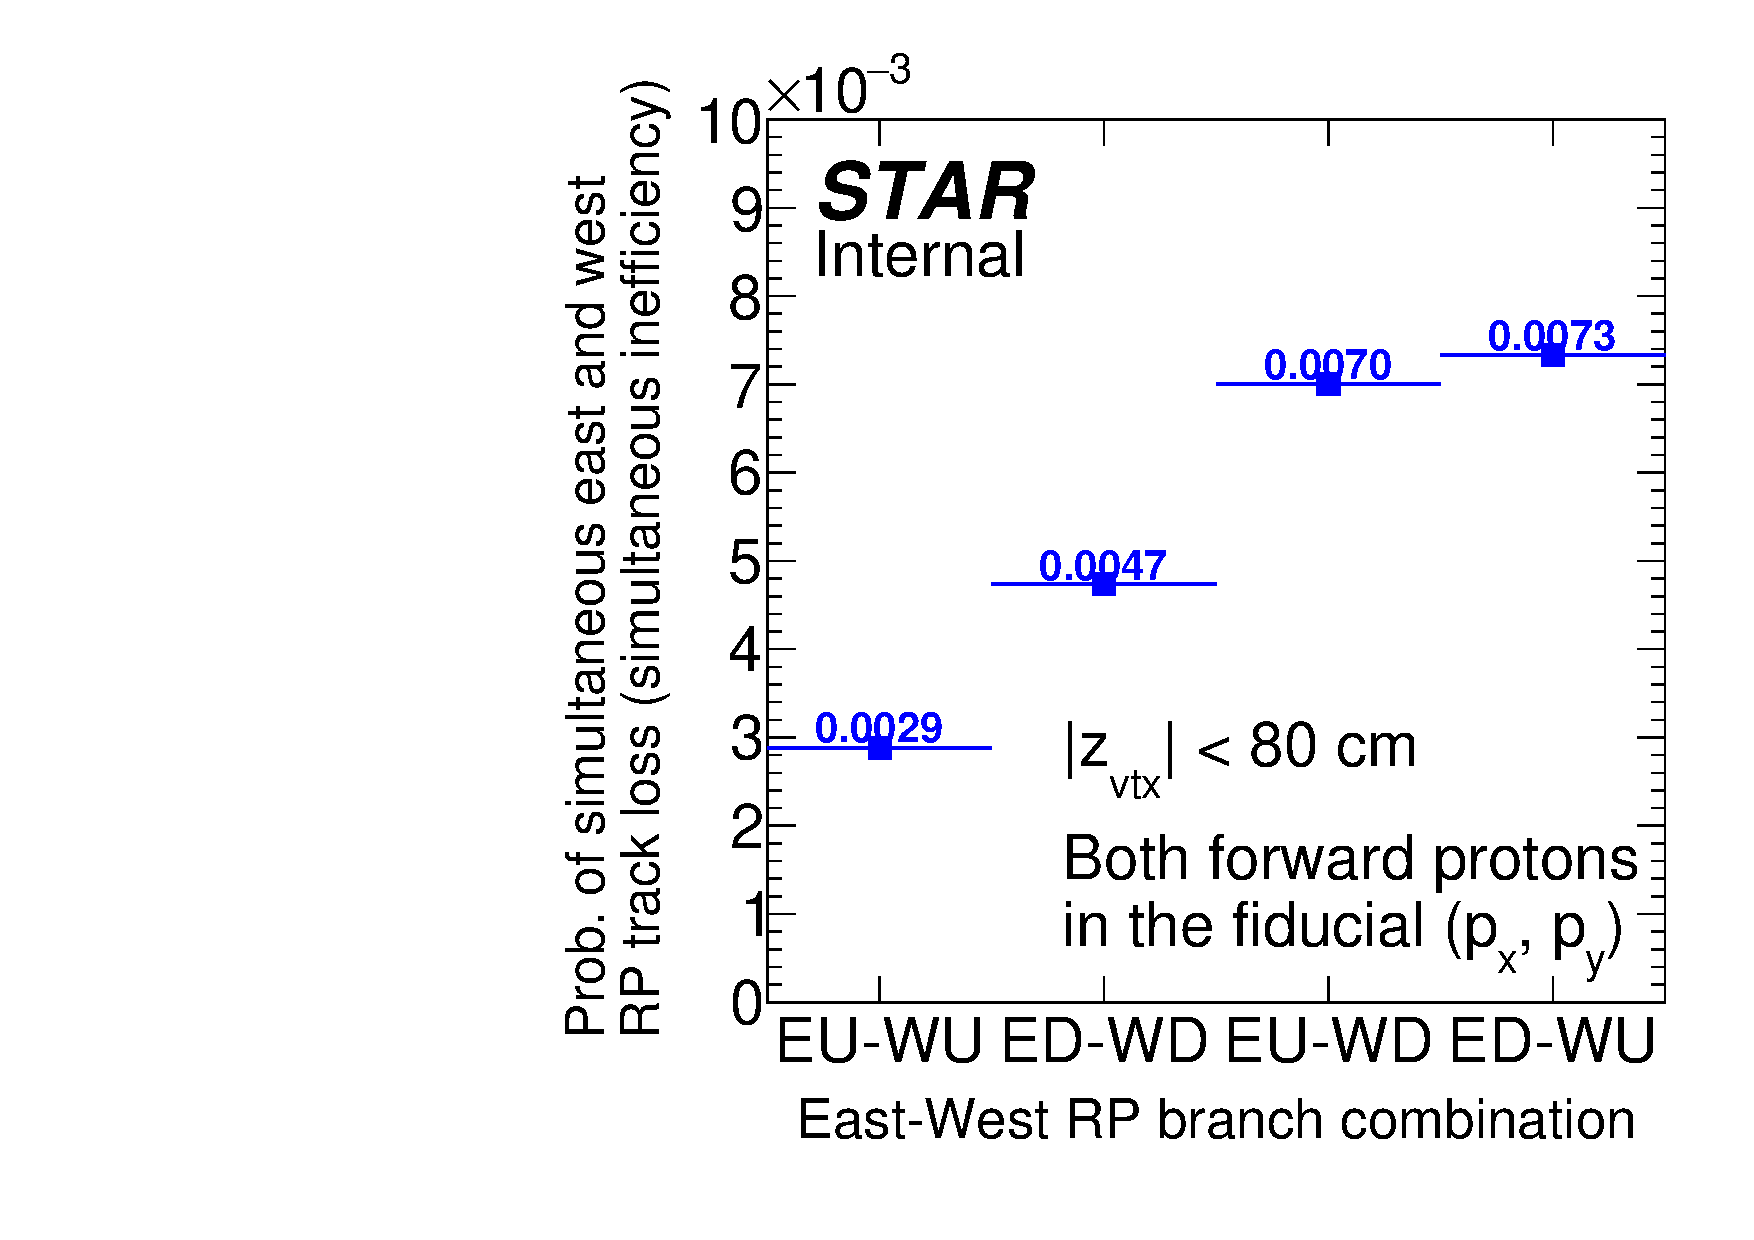
\includegraphics[width=\linewidth]{graphics/corrections/SimultaneousEastWestRpTrackLoss.pdf}%
  \caption{Probability of simultaneous inefficiency of the RP track reconstruction calculated from the CEP MC embedded into zero-bias data.\newline\newline\newline\newline\newline}\label{fig:SimultaneousEastWestRpTrackLoss}
\end{minipage}%
\end{figure}%
%---------------------------


The efficiency calculated in the way described above is, by design, the acceptance, reconstruction and selection efficiency for a single proton on one side of the IP. In CEP event there are two independent forward protons which may be simultaneously not reconstructed or rejected by the selection algorithm due to e.g. elastic pile-up interaction providing additional good quality proton tracks on both sides of IP. One could, in principle, calculate 5-dimensional efficiency for both forward protons (in variables $p_{x}^{\text{E}}, p_{y}^{\text{E}}, p_{x}^{\text{W}}, p_{y}^{\text{W}}$ and $z_{\text{vtx}}$) which would ultimately account for the simultaneous east and west inefficiency, however this would require orders of magnitude larger statistics of MC to provide reasonably low statistical uncertainty of the efficiency. Instead, on top of the 3-dimensional reconstruction and selection efficiencies for east and west RPs we calculate (from embedded MC) probability that the proton tracks are simultaneously not reconstructed or selected on the east and west side, despite the trigger signal solely in expected RP branches (no trigger veto) and true-level $(p_{x}, p_{y})$ of both forward protons contained in the fiducial region. This probability, denoted as
\begin{equation}
\mathcal{P}^{\text{E\&W}}_{\text{loss}} = \mbox{\LARGE$\varepsilon$}\left(!\RPE\land~!\RPW\Big|\TRE\land\TRW\land~!\V\Big.\right),
\end{equation}
 is presented in Fig.~\ref{fig:SimultaneousEastWestRpTrackLoss} for all four comibnations of east and west RP branches.





\subsection{TPC vertex reconstruction efficiency}\label{sec:tpcVxRecoEff}

The definition of vertex reconstruction efficiency established in this analysis is the probability that two global tracks, both associated with true-level primary particles from the kinematic region of the measurement, both satisfying kinematic and quality criteria (cuts~\ref{enum:TpcKinematicCuts} and ~\ref{enum:TpcQualityCuts}) and both matched with hits in TOF, form a vertex listed in the collection of reconstructed primary vertices and DCA(R) and DCA(z) of both global tracks calculated w.r.t. this vertex is contained within the limits of cut~\ref{enum:TpcDcaCuts}.

\section{Particle energy loss}\label{sec:energyLoss}

Energy loss correction as a function of reconstructed particle $p_{T}$ in bins of $z$-position of reconstructed vertex has been calculated and presented in Chapter~5 of Ref.~\cite{supplementaryNote} for all analyzed particle species and both positive and negative charges. The correction was applied independetly for each particle in the following procedure:

\begin{enumerate}
	\item After central particles were identified (cut~\ref{enum:CutPid}) an absolute value of the particle transverse momentum correction ($-\Delta p_{T} = p_{T}^{\text{meas}}-p_{T}^{\text{true}}$) was read from the histogram corresponding to reconstructed $z_{\text{vtx}}$ and to assigned particle ID (Appendix~C of Ref.~\cite{supplementaryNote}).
	\item The momentum correction factor $f_{p}^{\text{corr}}$ was calculated:
	\begin{equation}\label{eq:pCorrFactor}
 f_{p}^{\text{corr}} = \frac{p_{T}^{\text{meas}} + \Delta p_{T}}{p_{T}^{\text{meas}}}.
  \end{equation}
  \item New, corrected momentum $\vec{p}^{corr}$ was assigned to the particle:
  \begin{equation}
   \vec{p}^{~\text{corr}} = f_{p}^{\text{corr}} \cdot \vec{p}^{~\text{meas}}.
  \end{equation}
  In this way all three components of particle momentum are corrected so that the pseudorapidity of a particle remains unchanged.
\end{enumerate}
This new momentum was further used in determination of total transverse momentum of all reconstructed particles, $p_{T}^{\text{miss}}$, as well as in applying TPC and TOF efficiency corrections and preparing histograms (cross sections) of physics quantities (e.g. invariant mass, rapidity of a pair of central tracks).


\section{Background subtraction}\label{sec:bkgdSubtraction}
% \section{Unfolding}\label{sec:unfolding}

% 
%   W analizie CEP wydajnosc werteksowania to prawdopodobieństwo że
%  oba pierwotne slady z punktu B tworza werteks (to znaczy sa na liscie
%  sladow primary wspolnego werteksu i spelniaja ciecia DCA).
%  Nie patrzymy na dodatkowe werteksy, hity w TOF, BBC_small
% 
% E) --- pozostale wydajnosci
% 
%   w przypadku analizy CEP jest to pile-up czyli dodatkowy werteks lub
%   dodatkowy hit w TOF lub sygnal w BBC. Te poprawk mamy z embeddingu
%   patrzac ile przypadkow z D ma dodatkowy werteks, hist w TOF lub BBC
% 
%   To samo powinnismy dostac z analizy "naszych" zero-bias.
% 
%   W przypadku analizy SD mamy pile-up czyli dodatkowy werteks, BBC
%   po stronie protonu też to znamy z embeddingu lub "naszych" zero-bias.
% 
%   Dodatkowo dochodza dodatkowe werteksy z oddzialywań wtornych/rozpadow.
%   Ten efekt znamy z MC. Powinno byc to samo z pile-up'em jak i  bez
% 
% 
% Jakies uwagi?
